%!TEX root = thesis.tex

\chapter{Results: Time-to-fix} % (fold)
\label{cha:results_time_to_fix}

In this chapter, the second research question and the accompanying hypotheses are investigated, as defined in Section~\ref{sec:research_questions}:

\vspace{\baselineskip}
\questionb{}

In order to answer this question, the following hypothesis are stated:

\vspace{\baselineskip}
\hypba{}

\vspace{\baselineskip}
\hypbb{}

\vspace{\baselineskip}
\hypbc{}

\section{Overview} % (fold)
All investigations are split into three parts: 
\begin{inparaenum}[(1)]
\item \textbf{results}, describing the direct results of the study and showing some descriptive statistics,
\item \textbf{analysis}, analysing the results of the study, and
\item \textbf{conclusions}, which evaluates the hypothesis.
\end{inparaenum}

In Section \ref{sec:analysis_of_ttf_vs_presence_of_stack_trace_in_bug_report}, it is investigated whether the time-to-fix of a bug decreases when a stack trace is present. Section \ref{sec:analysis_of_ttf_version_stack_trace_position_in_comments} investigates if the position of a stack trace in the bug report has influence on the time-to-fix. Section \ref{sec:correlation_analysis_between_loc_and_ttf} investigates the correlation between class size and the time-to-fix of the corresponding bug reports.

Finally, all results found in the previous mentioned sections are summarised in Section \ref{sec:ttf_summary_of_results}.

% section overview (end)

\section{Analysis of time-to-fix versus presence of stack traces in bug report} % (fold)
\label{sec:analysis_of_ttf_vs_presence_of_stack_trace_in_bug_report}
We expect that the time-to-fix of a bug decreases when a stack trace is present in the bug report. With this stack trace, it might be easier to reproduce the bug and to know where to look in the source code. This is also shown by Schr\"{o}ter \emph{et al.} in \cite{Schroter2010}. Therefore, the first hypothesis of research question R1 is investigated in this section:

\vspace{\baselineskip}
\hypba{}

\subsection{Results} % (fold)
All bug reports from \texttt{jdt.debug} marked with status \textsc{verified} and resolution \textsc{fixed} are split into two groups: 

\begin{enumerate*}
	\item bug reports that include a stack trace in one or more of the comments, and
	\item bug reports that do not include a stack trace.
\end{enumerate*}

All bugs from \texttt{jdt.core} are discarded, since only a specific subset of bugs is imported (the bugs that probably mention one or more exceptions). This means this specific data set is expected to have a certain bias. Although not all imported bugs do contain an actual exception, which might make the data set usable after all, we decided to not use this data set in our investigations.

For each bug report, the time-to-fix is calculated. All reports with a time-to-fix of $0$ days are removed from the data sets, since these reports probably are only created for administrative reasons.

In Table~\ref{tab:ttf_stats}, some descriptive statistics of the resulting data sets are shown, such as mean, standard deviation, minimum value, maximum value and median. The data sets are also plotted as box plots in Figure~\ref{fig:ttf_with_without_stacktrace}.

\begin{table}[!ht]\footnotesize
	\centering
	\begin{tabular}{lrrrrrr}
		\toprule
		data set & N & min & max & mean & median & std \\
		\midrule
		\texttt{jdt.debug} with stack trace & 180 & 1 & 644 & 62 & 14 & 108 \\
		\texttt{jdt.debug} without stack trace & 2,108 & 1 & 3,137 & 98 & 18 & 232 \\
		\bottomrule
	\end{tabular} 
	\caption{Time-to-fix (in days) statistics of the jdt.debug. N is the number of measurements.}
	\label{tab:ttf_stats}
\end{table}
 
\begin{figure}[!ht]
	\centering
		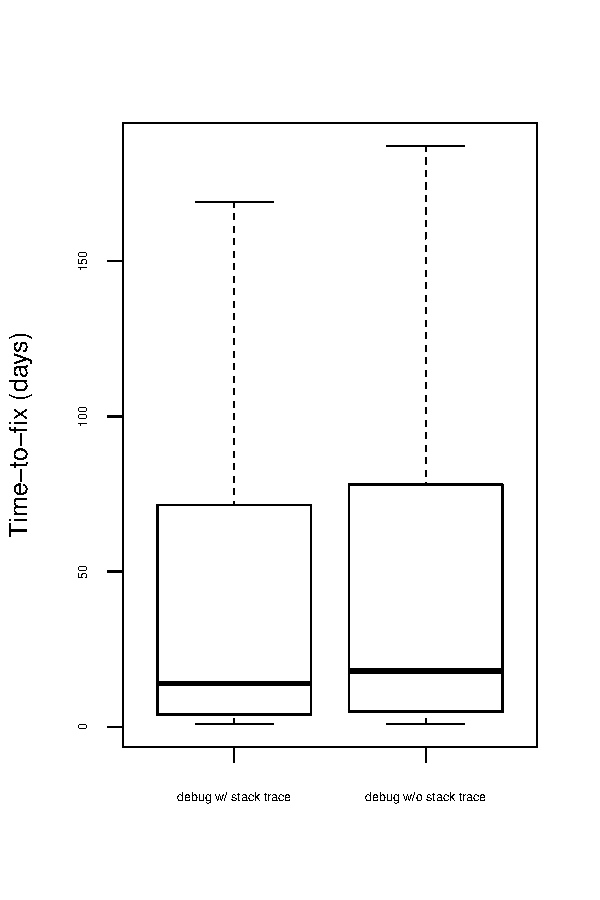
\includegraphics[width=0.7\textwidth]{img/ttf_with_without_stacktrace.pdf}
	\caption{Comparison between bug reports with and without a stack trace (whiskers at 1.5 times the IQR).}
	\label{fig:ttf_with_without_stacktrace}
\end{figure}

% subsection results (end)

\subsection{Analysis} % (fold)
We are investigating if the time-to-fix of a bug decreases when a stack trace is present in the bug report. In order to do this, the median time-to-fix for data sets with and without stack traces are compared. This is done pairwise for the \texttt{jdt.debug} project.

Table~\ref{tab:ttf_stats} shows that for \texttt{jdt.debug}, the median time-to-fix decreases when a stack trace is present. The mean time-to-fix decreases by five weeks when a stack trace is present.

Since the data sets are not normal distributed and the distributions of the data sets are similar shaped (see Appendix~\ref{sub:norm:presence_of_stack_trace}), the Wilcoxon Rank Sum test (see Section~\ref{sub:wilcoxon_rank_sum_test}) is used to compare the medians of the data sets.
The null hypothesis for the Wilcoxon test states that the median values of two data sets does not differ. The alternative hypothesis for the one-sided test states $M_1 < M_2$, where $M_i$ is the median of group $i$. 

The $p$-value for this one-sided Wilcoxon Rank Sum test for \texttt{jdt.debug} is:

\[
	p = 0.1277
\]

% subsection analysis (end)

\subsection{Conclusions} % (fold)
When looking at the time-to-fix statistics in Table~\ref{tab:ttf_stats}, it can be noted the median time-to-fix decreases when a stack trace is mentioned in a bug report. Also, the mean time-to-fix decreases by five weeks when a stack trace is present. 

With respect to the mean time-to-fix, a higher standard deviation can be noticed in the data sets without stack traces. This, combining with a relative higher number of measurements (and thus probably a higher number of outliers, since the distributions are similar), causes the increase in time-to-fix.

Based on the results of the one-sided Wilcoxon test, the $p$-value for \texttt{jdt.debug} does not satisfy $p < \alpha$, where $\alpha = 0.05$. Therefore we conclude that there is no evidence that the median time-to-fixes in bug reports with a stack trace differs from bug reports without a stack trace. However, the descriptive statistics are promising, showing that both mean (over a month) and median (4 days) time-to-fix values decrease significantly when a stack trace is present. We therefore partially accept hypothesis H2.1:

\vspace{\baselineskip}
\hypba{}

% subsection conclusions (end)
% section analysis_of_ttf_vs_presence_of_stack_trace_in_bug_report (end)

\section{Analysis of time-to-fix versus stack trace position in comments} % (fold)
\label{sec:analysis_of_ttf_version_stack_trace_position_in_comments}
The previous section showed there is no evidence for a decrease in time-to-fix when a stack trace is present. However, could the time-to-fix be positively affected (i.e., decrease) when the stack trace is present in the \emph{first} comment of a bug report? This way, the stack trace is immediately available to the bug traiger, and can therefore be used in the assessment of the bug report. In this section, the second hypothesis of research question R2 is investigated:

\vspace{\baselineskip}
\hypbb{}

\subsection{Results} % (fold)
All bug reports with a stack trace from \texttt{jdt.core} and \texttt{jdt.debug} marked with status \textsc{verified} and resolution \textsc{fixed} are split into two groups: 

\begin{enumerate*}
	\item bug reports with one or more stack traces in the first comment, and
	\item bug reports with one or more stack traces in non-first comment(s).
\end{enumerate*}

For each bug report, the time-to-fix is calculated. All reports with a time-to-fix of $0$ days are removed from the data sets, since these reports probably are only created for administrative reasons.

In Table~\ref{tab:ttf_pos_stats}, some descriptive statistics of the resulting data sets are shown, such as mean, standard deviation, minimum value, maximum value and median. The data sets are also plotted as box plots in Figure~\ref{fig:ttf_pos_stats}.

\begin{table}[!ht]\footnotesize
	\centering
	\begin{tabular}{lrrrrrr}
		\toprule
		data set & N & min & max & mean & median & std \\
		\midrule
		\texttt{jdt.debug} with stack traces in first comment & 116 & 1 & 1,744 & 60 & 9 & 178 \\
		\texttt{jdt.debug} with stack traces in non-first comment(s) & 23 & 1 & 1,130 & 137 & 40 & 209 \\
		\texttt{jdt.core} with stack traces in first comment & 186 & 1 & 644 & 66 & 12 & 119 \\
		\texttt{jdt.core} with stack traces in non-first comment(s) & 52 & 1 & 285 & 57 & 29 & 87 \\
		overall with stack traces in first comment & 302 & 1 & 1,744 & 62 & 12 & 157 \\
		overall with stack traces in non-first comment(s) & 75 & 1 & 1,130 & 112 & 32 & 184 \\
		\bottomrule
	\end{tabular} 
	\caption{Time-to-fix (in days) statistics of the data. N is the number of measurements.}
	\label{tab:ttf_pos_stats}
\end{table}
 
\begin{figure}[!ht]
	\centering
		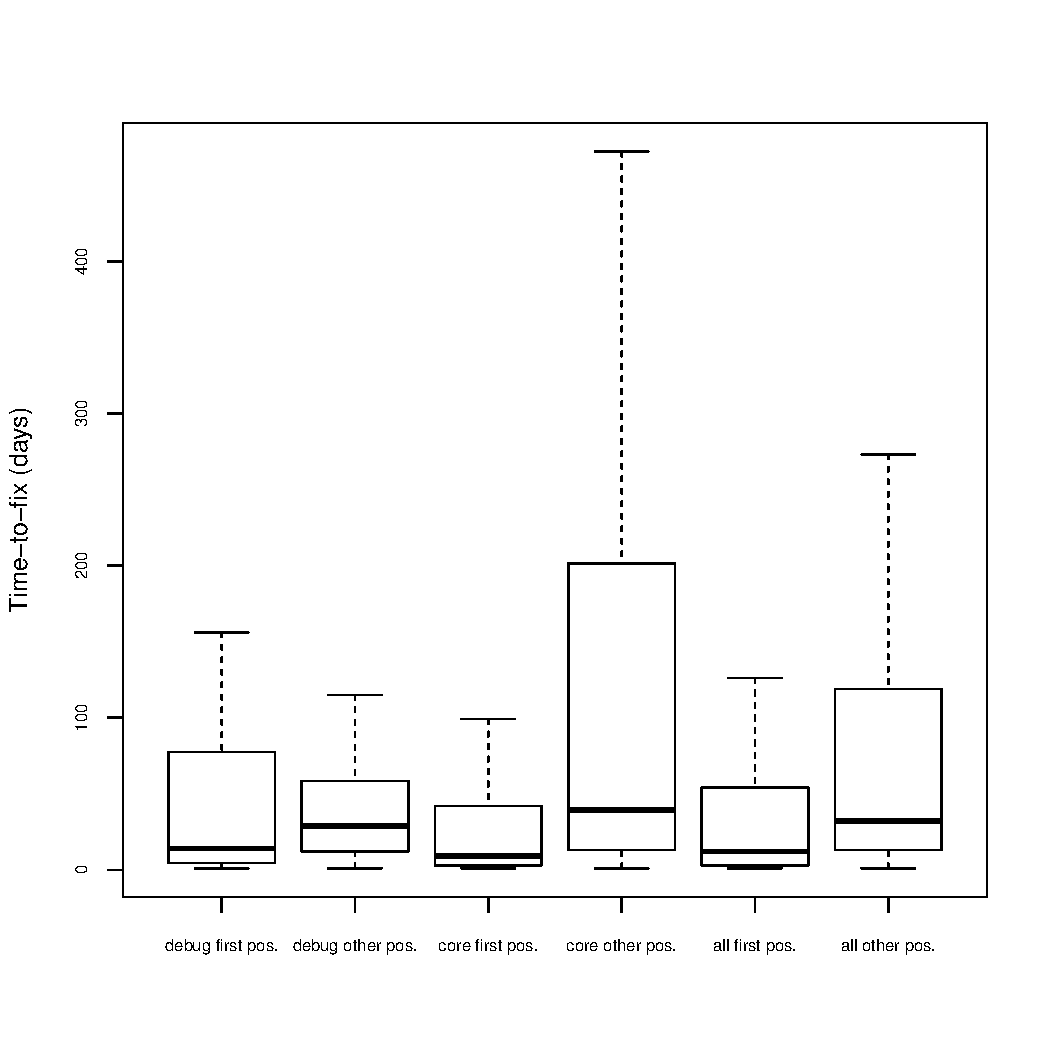
\includegraphics[width=1\textwidth]{img/ttf_stacktrace_pos.pdf}
	\caption{Comparison between bug reports with and without a stack trace (whiskers at 1.5 times the IQR).}
	\label{fig:ttf_pos_stats}
\end{figure}

% subsection results (end)

\subsection{Analysis} % (fold)
We are investigating if the time-to-fix of a bug report that includes one or more stack traces \emph{decreases} when a stack trace is present in the first comment of the bug report. In order to do this, the median time-to-fix for these data sets are compared:

\begin{itemize*}
	\item \texttt{jdt.debug} reports with stack traces in the first comment versus \texttt{jdt.debug} reports with stack traces in non-first comments
	\item \texttt{jdt.core} reports with stack traces in the first comment versus \texttt{jdt.core} reports with stack traces in non-first comments
	\item combined bug reports from \texttt{jdt.debug} and \texttt{jdt.core} with stack traces in the first comment versus combined bug reports from \texttt{jdt.debug} and \texttt{jdt.core} with stack traces in non-first comments
\end{itemize*}

Table~\ref{tab:ttf_pos_stats} shows that for all data sets, the median time-to-fix decreases when a stack trace is present in the first comment. In all three measures, the mean time-to-fix decreases by two to four weeks. 

Since the data sets are not normal distributed and the distributions of the data sets are similar shaped (see Appendix~\ref{sub:norm:presence_of_stack_trace}), the Wilcoxon Rank Sum test (see Section~\ref{sub:wilcoxon_rank_sum_test}) is used to compare the medians of the data sets.
The null hypothesis for the Wilcoxon test states that the median values of two data sets does not differ. The alternative hypothesis for the one-sided test states $M_1 < M_2$, where $M_i$ is the median of group $i$. The results of the one-sided Wilcoxon Rank Sum test between the data sets are given in Table~\ref{tab:wilcoxon_pos}.

\begin{table}[!ht]\footnotesize
	\centering
	\begin{tabular}{llrl}
		\toprule
		data set 1 & data set 2 & $p$-value & \\
		\midrule
		\texttt{jdt.debug} w/ st. in first comment & \texttt{jdt.debug} w/ st. in other comment & $0.1271$ & \\
		\texttt{jdt.core} w/ st. in first comment & \texttt{jdt.core} w/ st. in other comment & $< 0.001$ & *** \\
		overall  w/ st. in first comment & overall w/ st. in other comment & $< 0.001$ & *** \\
		\bottomrule
	\end{tabular} 
	\caption{One-sided Wilcoxon test results.}
	\label{tab:wilcoxon_pos}
\end{table}

% subsection analysis (end)

\subsection{Conclusions} % (fold)
When looking at the time-to-fix statistics in Table~\ref{tab:ttf_pos_stats}, it can be noted the median time-to-fix decreases decreases when a stack trace is present in the first comment. Based on the results of the one-sided Wilcoxon test in Table~\ref{tab:wilcoxon_pos}, the $p$-values for \texttt{jdt.core} and the overall data set satisfy $p < \alpha$, where $\alpha = 0.001$, resulting in a highly significant result. However, for \texttt{jdt.debug}, no statistically significant $p$-value is found, which is probably due to the fact that the number of data points is limited.

In conclusion, the null hypothesis stating the difference in medians of the two data sets is a coincidence is rejected for \texttt{jdt.core} and the overall data set. Therefore, there is evidence that the time-to-fix for bugs decreases when a stack trace is present in the first comment, compared to bug reports with a stack trace in the non-first comment. We therefore accept hypothesis H2.2:

\vspace{\baselineskip}
\hypbb{}

\noindent
This is consistent with the results of Schr\"{o}ter \emph{et al.} \cite{Schroter2010}. They found strong evidence that bug reports that include one or more stack traces do indeed have a shorter lifetime. Regarding stack trace position in the bug report, they found that 70\% of the bugs were fixed in a stack frame from the \emph{first} stack trace in the bug report.

% subsection conclusions (end)

% section analysis_of_ttf_version_stack_trace_position_in_comments (end)

\section{Correlation analysis between class size and time-to-fix} % (fold)
\label{sec:correlation_analysis_between_loc_and_ttf}
When one or more stack traces are present in comments of a bug report, it is possible to relate each bug report to one or more source classes. A larger class size might point to less understandable code, hence to a higher time-to-fix for a bug. In this section, it will be investigated if there is a relation between class size and time-to-fix of a bug report. The following hypothesis of research question R2 will be discussed:

\vspace{\baselineskip}
\hypbc{}

\subsection{Results} % (fold)
Table~\ref{tab:ttf_loc_stats} contains all 29 classes in both the \texttt{jdt.debug} and \texttt{jdt.core} projects that are matched to at least ten bug reports with status \textsc{verified} and resolution \textsc{fixed}. We match to at least ten bug reports, so we are sure the descriptive statistics are based on sufficient data. All bug reports with a fix time of 0 days are again removed from the results. For each class, the number of matching bug reports, the median time-to-fix of these bug reports, and the lines of code of the class are shown.

The total number of distinct classes in all stack traces is 2,533, but only 339 (13\%) from these classes are available as actual source code for \texttt{jdt.debug} or \texttt{jdt.core}. All other classes refer to classes from external libraries or the Java core. From these 339 classes, only the 29 (8\%, 1\% overall) classes shown in Table~\ref{tab:ttf_loc_stats} are mentioned in ten or more bug reports.

\begin{table}[!ht]\footnotesize
	\centering
	\begin{tabular}{lr|rrrrrr}
		\toprule
		class & LOC & N & min & max & mean & med. & std \\
		\midrule
		\verb|core.dom.ASTParser| & 593 & 12 & 3 & 366 & 53 & 14 & 106 \\
		\verb|core.JavaCore| & 1,309 & 14 & 2 & 366 & 105 & 57 & 116 \\
		\verb|core.search.SearchEngine| & 286 & 20 & 1 & 1,161 & 160 & 34 & 288 \\
		\verb|internal.codeassist.CompletionEngine| & 10,833 & 11 & 1 & 449 & 54 & 7 & 132 \\
		\verb|i.comp.ast.AbstractMethodDeclaration| & 364 & 14 & 1 & 149 & 18 & 8 & 38 \\
		\verb|i.comp.ast.CompilationUnitDeclaration| & 559 & 19 & 1 & 149 & 18 & 7 & 35 \\
		\verb|i.comp.ast.MethodDeclaration| & 217 & 14 & 1 & 244 & 29 & 7 & 64 \\
		\verb|i.comp.ast.TypeDeclaration| & 1,108 & 25 & 1 & 244 & 26 & 8 & 55 \\
		\verb|i.comp.Compiler| & 580 & 36 & 1 & 150 & 26 & 9 & 43 \\
		\verb|i.comp.lookup.ClassScope| & 998 & 11 & 1 & 150 & 33 & 11 & 51 \\
		\verb|i.comp.lookup.CompilationUnitScope| & 654 & 16 & 1 & 150 & 25 & 9 & 43 \\
		\verb|i.comp.lookup.LookupEnvironment| & 1,015 & 16 & 1 & 150 & 26 & 10 & 43 \\
		\verb|i.comp.lookup.Scope| & 3,297 & 12 & 1 & 150 & 31 & 8 & 49 \\
		\verb|i.core.BinaryType| & 740 & 11 & 1 & 1,744 & 201 & 40 & 514 \\
		\verb|i.core.builder.AbstractImageBuilder| & 641 & 14 & 1 & 147 & 26 & 12 & 39 \\
		\verb|i.core.builder.JavaBuilder| & 639 & 16 & 1 & 147 & 24 & 10 & 37 \\
		\verb|i.core.CompilationUnit| & 877 & 35 & 1 & 449 & 60 & 9 & 105 \\
		\verb|i.core.CompilationUnitProblemFinder| & 162 & 19 & 1 & 253 & 41 & 9 & 71 \\
		\verb|i.core.JavaElement| & 534 & 29 & 1 & 1,744 & 125 & 36 & 324 \\
		\verb|i.core.JavaModelManager| & 3,749 & 13 & 5 & 243 & 59 & 30 & 78 \\
		\verb|i.core.JavaModelOperation| & 553 & 34 & 1 & 266 & 56 & 13 & 84 \\
		\verb|i.core.JavaProject| & 2,087 & 19 & 1 & 253 & 65 & 30 & 84 \\
		\verb|i.core.Openable| & 311 & 24 & 1 & 449 & 71 & 11 & 117 \\
		\verb|i.core.ReconcileWorkingCopyOperation| & 173 & 22 & 1 & 253 & 47 & 8 & 80 \\
		\verb|i.core.search.BasicSearchEngine| & 1,285 & 15 & 1 & 1,161 & 192 & 51 & 324 \\
		\verb|i.core.search.JavaSearchParticipant| & 46 & 13 & 1 & 1,161 & 166 & 13 & 341 \\
		\verb|i.core.search.matching.MatchLocator| & 2,273 & 17 & 1 & 1,161 & 134 & 17 & 292 \\
		\verb|i.core.search.processing.JobManager| & 357 & 11 & 1 & 576 & 120 & 15 & 204 \\
		\verb|internal.debug.core.model.JDIThread| & 1,467 & 19 & 1 & 349 & 72 & 19 & 106 \\
		\bottomrule
	\end{tabular} 
	\caption{Line of code and time-to-fix (in days) statistics for classes. (All classes are in org.eclipse.jdt, i.comp = internal.compiler, i.core = internal.core). N is the number of measurements.}
	\label{tab:ttf_loc_stats}
\end{table}

To visualise a possible correlation between time-to-fix and class size, Figure~\ref{fig:ttf_loc_scatter} depicts a scatter plot of these two variables. On the x-axis, the median time-to-fix of all corresponding issues for a class is shown, where on the y-axis, the lines of code for this class is shown. The green solid line depicts a linear regression line, where the red solid line is a non-parametric Loess \cite{Cleveland1979,Cleveland1988} regression line. The Loess regression line is non-parametric, which means it does not make an assumption about the form of the relationship between time-to-fix and class size. Also, on both axis, a box plot is drawn to show the distribution of the data points.

\begin{figure}[!ht]
	\centering
		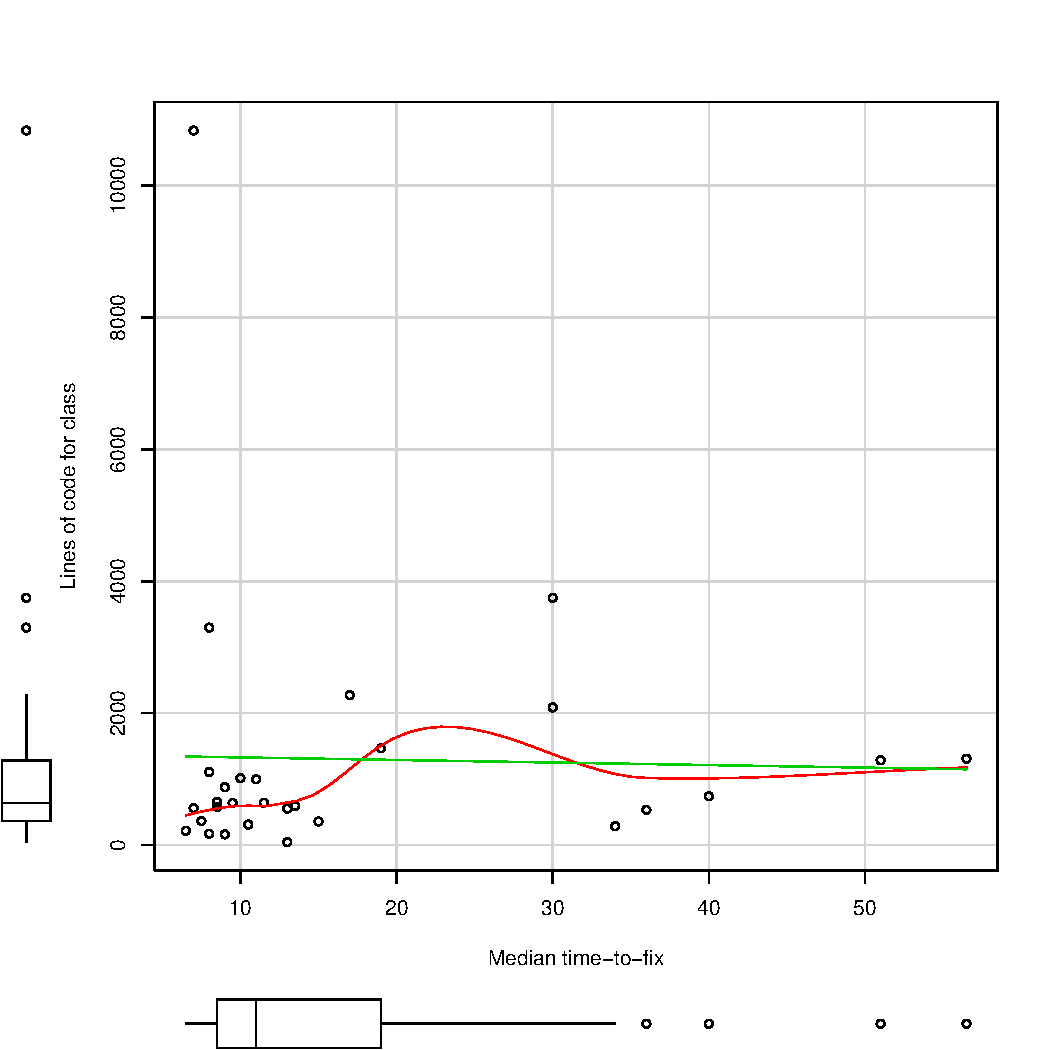
\includegraphics[width=1\textwidth]{img/ttf-classes-loc.pdf}
	\caption{Scatter plot of time-to-fix vs lines of code. On the x-axis, the median time-to-fix of all corresponding issues for a class is shown, where on the y-axis, the lines of code of the class are shown. The green solid line depicts a linear regression line, where the red solid line is a non-parametric Loess regression line ($f = 0.7$).}
	\label{fig:ttf_loc_scatter}
\end{figure}

% subsection results (end)

\subsection{Analysis} % (fold)
As can be seen in Figure~\ref{fig:ttf_loc_scatter}, no evident visual signs of correlation can be noticed between median time-to-fix and the corresponding class size. In order to statistically verify if a correlation is present, the Kendall tau-b rank correlation coefficient ($\tau_B$) is calculated. When the Kendall tau-b test (see Section~\ref{sub:kendall_tau_b_rank_correlation_coefficient}) is applied to the data set, the following $\tau_B$ value is found:

\begin{equation}
	\tau_B = 0.129
\end{equation}

The null hypothesis for the Kendall tau-b test states `there is no relationship between the two variables'. Since $\tau_B = 0.129$, a weak correlation can be expected to exists between the two variables. However, for this $\tau_B$, a $p$-value of 0.338 is found, meaning the null hypothesis that that the variables are statistically independent cannot be rejected. This large $p$-value is probably caused by the low number of data points and several outliers in the dataset.

% subsection analysis (end)

\subsection{Conclusions} % (fold)
The data set only has 29 data points due to the fact that not much bug reports have 10 or more matching classes. This is a limitation for the correlation analysis. As can be seen in the scatter plot in Figure~\ref{fig:ttf_loc_scatter}, no apparent correlation is shown. The Kendall tau-b test does not give a statistical significant result, meaning the null hypothesis that that the variables are statistically independent cannot be rejected. In conclusion, it is not possible to accept or reject hypothesis H2.3: 

\vspace{\baselineskip}
\hypbc{}

% subsection conclusions (end)

% section correlation_analysis_between_loc_and_ttf (end)

\section{Summary of results} % (fold)
\label{sec:ttf_summary_of_results}
This chapter showed the results and analysis for research question R2, as described in Chapter~\ref{sec:analysis:time_to_fix}:

\vspace{\baselineskip}
\questionb{}
\vspace{\baselineskip}

\noindent
First, it was investigated whether the time-to-fix of a bug decreases if a stack trace is present. A comparison between bug reports with and without a stack trace shows no difference between the median time-to-fix values. However, the descriptive statistics are promising, showing that both mean and median time-to-fix values decrease significantly when a stack trace is present. We therefore partially accept hypothesis H2.1.

Next, it was investigated if the time-to-fix decreases when a stack trace is present in the first comment of a bug report (compared to a trace in other comments). When comparing the median time-to-fix values again, a significant result is found. Hypothesis H2.2 therefore is accepted.

Finally, a possible relationship between class size and time-to-fix is investigated. Due to the limited amount of data available, it is not possible to state anything regarding hypothesis H2.3.
% section summary_of_results (end)

% chapter results_time_to_fix (end)